\documentclass[twoside]{book}

% Packages required by doxygen
\usepackage{calc}
\usepackage{doxygen}
\usepackage{graphicx}
\usepackage[utf8]{inputenc}
\usepackage{makeidx}
\usepackage{multicol}
\usepackage{multirow}
\usepackage{fixltx2e}
\PassOptionsToPackage{warn}{textcomp}
\usepackage{textcomp}
\usepackage[nointegrals]{wasysym}
\usepackage[table]{xcolor}

% Font selection
\usepackage[T1]{fontenc}
\usepackage{mathptmx}
\usepackage[scaled=.90]{helvet}
\usepackage{courier}
\usepackage{amssymb}
\usepackage{sectsty}
\renewcommand{\familydefault}{\sfdefault}
\allsectionsfont{%
  \fontseries{bc}\selectfont%
  \color{darkgray}%
}
\renewcommand{\DoxyLabelFont}{%
  \fontseries{bc}\selectfont%
  \color{darkgray}%
}
\newcommand{\+}{\discretionary{\mbox{\scriptsize$\hookleftarrow$}}{}{}}

% Page & text layout
\usepackage{geometry}
\geometry{%
  a4paper,%
  top=2.5cm,%
  bottom=2.5cm,%
  left=2.5cm,%
  right=2.5cm%
}
\tolerance=750
\hfuzz=15pt
\hbadness=750
\setlength{\emergencystretch}{15pt}
\setlength{\parindent}{0cm}
\setlength{\parskip}{0.2cm}
\makeatletter
\renewcommand{\paragraph}{%
  \@startsection{paragraph}{4}{0ex}{-1.0ex}{1.0ex}{%
    \normalfont\normalsize\bfseries\SS@parafont%
  }%
}
\renewcommand{\subparagraph}{%
  \@startsection{subparagraph}{5}{0ex}{-1.0ex}{1.0ex}{%
    \normalfont\normalsize\bfseries\SS@subparafont%
  }%
}
\makeatother

% Headers & footers
\usepackage{fancyhdr}
\pagestyle{fancyplain}
\fancyhead[LE]{\fancyplain{}{\bfseries\thepage}}
\fancyhead[CE]{\fancyplain{}{}}
\fancyhead[RE]{\fancyplain{}{\bfseries\leftmark}}
\fancyhead[LO]{\fancyplain{}{\bfseries\rightmark}}
\fancyhead[CO]{\fancyplain{}{}}
\fancyhead[RO]{\fancyplain{}{\bfseries\thepage}}
\fancyfoot[LE]{\fancyplain{}{}}
\fancyfoot[CE]{\fancyplain{}{}}
\fancyfoot[RE]{\fancyplain{}{\bfseries\scriptsize Generated on Thu Jul 17 2014 21\+:19\+:47 for Touch Screen Geometry by Doxygen }}
\fancyfoot[LO]{\fancyplain{}{\bfseries\scriptsize Generated on Thu Jul 17 2014 21\+:19\+:47 for Touch Screen Geometry by Doxygen }}
\fancyfoot[CO]{\fancyplain{}{}}
\fancyfoot[RO]{\fancyplain{}{}}
\renewcommand{\footrulewidth}{0.4pt}
\renewcommand{\chaptermark}[1]{%
  \markboth{#1}{}%
}
\renewcommand{\sectionmark}[1]{%
  \markright{\thesection\ #1}%
}

% Indices & bibliography
\usepackage{natbib}
\usepackage[titles]{tocloft}
\setcounter{tocdepth}{3}
\setcounter{secnumdepth}{5}
\makeindex

% Hyperlinks (required, but should be loaded last)
\usepackage{ifpdf}
\ifpdf
  \usepackage[pdftex,pagebackref=true]{hyperref}
\else
  \usepackage[ps2pdf,pagebackref=true]{hyperref}
\fi
\hypersetup{%
  colorlinks=true,%
  linkcolor=blue,%
  citecolor=blue,%
  unicode%
}

% Custom commands
\newcommand{\clearemptydoublepage}{%
  \newpage{\pagestyle{empty}\cleardoublepage}%
}


%===== C O N T E N T S =====

\begin{document}

% Titlepage & ToC
\hypersetup{pageanchor=false,
             bookmarks=true,
             bookmarksnumbered=true,
             pdfencoding=unicode
            }
\pagenumbering{roman}
\begin{titlepage}
\vspace*{7cm}
\begin{center}%
{\Large Touch Screen Geometry }\\
\vspace*{1cm}
{\large Generated by Doxygen 1.8.7}\\
\vspace*{0.5cm}
{\small Thu Jul 17 2014 21:19:47}\\
\end{center}
\end{titlepage}
\clearemptydoublepage
\tableofcontents
\clearemptydoublepage
\pagenumbering{arabic}
\hypersetup{pageanchor=true}

%--- Begin generated contents ---
\chapter{Main Page}
\label{index}\hypertarget{index}{}Arduino library for creating geometries shapes for the Seeed Studio T\+F\+T touch screen (Version 1). \hypertarget{index_intro_sec}{}\section{Introduction}\label{index_intro_sec}
\begin{DoxyAuthor}{Author}
Richard Kirkpatrick 
\end{DoxyAuthor}
\begin{DoxyDate}{Date}
17 July 2014 
\end{DoxyDate}
\begin{DoxyCopyright}{Copyright}
G\+N\+U Public License.
\end{DoxyCopyright}
This is the Arduino library for creating geometries shapes for the Seeed Studio T\+F\+T touch screen (Version 1). The user can create polygons, rectangles, triangle and circles. See the Wiki documentation page for more info! 
\chapter{Hierarchical Index}
\section{Class Hierarchy}
This inheritance list is sorted roughly, but not completely, alphabetically\+:\begin{DoxyCompactList}
\item \contentsline{section}{Circle}{\pageref{class_circle}}{}
\item \contentsline{section}{Point2\+D}{\pageref{class_point2_d}}{}
\item \contentsline{section}{Point2\+D\+Array}{\pageref{class_point2_d_array}}{}
\item \contentsline{section}{Polygon}{\pageref{class_polygon}}{}
\begin{DoxyCompactList}
\item \contentsline{section}{Rectangle}{\pageref{class_rectangle}}{}
\item \contentsline{section}{Triangle}{\pageref{class_triangle}}{}
\end{DoxyCompactList}
\end{DoxyCompactList}

\chapter{Class Index}
\section{Class List}
Here are the classes, structs, unions and interfaces with brief descriptions\+:\begin{DoxyCompactList}
\item\contentsline{section}{\hyperlink{class_circle}{Circle} \\*The class for drawing circles to the T\+F\+T touch screen }{\pageref{class_circle}}{}
\item\contentsline{section}{\hyperlink{class_point2_d}{Point2\+D} \\*Abstract data type for representing a point in the 2\+D cartesian plane }{\pageref{class_point2_d}}{}
\item\contentsline{section}{\hyperlink{class_point2_d_array}{Point2\+D\+Array} \\*Abstract data class for arrays of \hyperlink{class_point2_d}{Point2\+D} objects }{\pageref{class_point2_d_array}}{}
\item\contentsline{section}{\hyperlink{class_polygon}{Polygon} \\*Base class for drawing \hyperlink{class_polygon}{Polygon} objects to the T\+F\+T touch screen }{\pageref{class_polygon}}{}
\item\contentsline{section}{\hyperlink{class_rectangle}{Rectangle} \\*Class for handling the geometry rendering and functions for the T\+F\+T Touch Screen }{\pageref{class_rectangle}}{}
\item\contentsline{section}{\hyperlink{class_triangle}{Triangle} \\*Class for drawing Triangles to the T\+F\+T touch screen }{\pageref{class_triangle}}{}
\end{DoxyCompactList}

\chapter{File Index}
\section{File List}
Here is a list of all documented files with brief descriptions\+:\begin{DoxyCompactList}
\item\contentsline{section}{\hyperlink{_touch_screen_geometry_8h}{Touch\+Screen\+Geometry.\+h} \\*Library for creating geometries shapes for the Seeed Studio T\+F\+T touch screen }{\pageref{_touch_screen_geometry_8h}}{}
\end{DoxyCompactList}

\chapter{Class Documentation}
\hypertarget{class_circle}{\section{Circle Class Reference}
\label{class_circle}\index{Circle@{Circle}}
}


The class for drawing circles to the T\+F\+T touch screen.  




{\ttfamily \#include $<$Touch\+Screen\+Geometry.\+h$>$}

\subsection*{Public Member Functions}
\begin{DoxyCompactItemize}
\item 
\hyperlink{class_circle_a88890d82b0634ae7c1f7395d0586d2bd}{Circle} (const \hyperlink{class_point2_d}{Point2\+D} \&my\+Centroid, const int my\+Radius, const unsigned int my\+Border\+Color=0xffff, const unsigned int my\+Fill\+Color=0x0000)
\begin{DoxyCompactList}\small\item\em Parameter constructor for the circle class. \end{DoxyCompactList}\item 
\hyperlink{class_circle_ab7a7dd06732d8519b3a2b14266952858}{Circle} (const int my\+X\+Start, const int my\+Y\+Start, const int my\+Radius, const unsigned int my\+Border\+Color=0xffff, const unsigned int my\+Fill\+Color=0x0000)
\begin{DoxyCompactList}\small\item\em Parameter constructor for the circle class. \end{DoxyCompactList}\item 
void \hyperlink{class_circle_a2f81a4869baba24481a710bbd266c395}{set\+Radius} (const int my\+Radius)
\begin{DoxyCompactList}\small\item\em Sets the radius of the circle. Does N\+O\+T redraw the circle. \end{DoxyCompactList}\item 
\hypertarget{class_circle_a4fee50b67efc5b5e188e92379140bb42}{const int \hyperlink{class_circle_a4fee50b67efc5b5e188e92379140bb42}{get\+Radius} ()}\label{class_circle_a4fee50b67efc5b5e188e92379140bb42}

\begin{DoxyCompactList}\small\item\em Gets the radius of the circle. \end{DoxyCompactList}\item 
void \hyperlink{class_circle_a2d0e705f07a4cb6a9d47eb759c73c59f}{set\+Border\+Color} (unsigned int my\+Border\+Color=0xffff)
\begin{DoxyCompactList}\small\item\em Sets the border color of the circle. \end{DoxyCompactList}\item 
void \hyperlink{class_circle_ab5f942fd85063fbb4bfc28fc4e700eca}{set\+Fill\+Color} (unsigned int=0x0000)
\begin{DoxyCompactList}\small\item\em Sets the fill color of the circle. \end{DoxyCompactList}\item 
\hypertarget{class_circle_ad6ce91ec588489091a42d02dda0b074a}{const unsigned int \hyperlink{class_circle_ad6ce91ec588489091a42d02dda0b074a}{get\+Border\+Color} ()}\label{class_circle_ad6ce91ec588489091a42d02dda0b074a}

\begin{DoxyCompactList}\small\item\em Gets the border color of the circle. \end{DoxyCompactList}\item 
const unsigned int \hyperlink{class_circle_a567e34480ed3af231bd019f66ab80fb7}{get\+Fill\+Color} ()
\begin{DoxyCompactList}\small\item\em Gets the fill color of the circle. \end{DoxyCompactList}\item 
\hypertarget{class_circle_a3a3f7166e7f629e44f9044b0e537eb22}{void \hyperlink{class_circle_a3a3f7166e7f629e44f9044b0e537eb22}{draw} ()}\label{class_circle_a3a3f7166e7f629e44f9044b0e537eb22}

\begin{DoxyCompactList}\small\item\em Uses the Seeed Studio T\+F\+T library to draw the circle. \end{DoxyCompactList}\item 
\hypertarget{class_circle_af69594749622c501d7a0c65715704e67}{void \hyperlink{class_circle_af69594749622c501d7a0c65715704e67}{fill} ()}\label{class_circle_af69594749622c501d7a0c65715704e67}

\begin{DoxyCompactList}\small\item\em Uses the Seeed Studio T\+F\+T library to fill the circle. \end{DoxyCompactList}\item 
void \hyperlink{class_circle_a73224ec141f6c58d1feff0a46a215b87}{move} (const int dx, const int dy)
\begin{DoxyCompactList}\small\item\em Moves the circle at the specified amount. Assumes the specified amount is not outside the screen boundaries. \end{DoxyCompactList}\item 
void \hyperlink{class_circle_ab02f952985bd988592c69409e2b5fe69}{scale} (const float factor)
\begin{DoxyCompactList}\small\item\em Resizes the circle based on the factor. Assumes the scaling factor is neither too small or too big. \end{DoxyCompactList}\end{DoxyCompactItemize}


\subsection{Detailed Description}
The class for drawing circles to the T\+F\+T touch screen. 

\subsection{Constructor \& Destructor Documentation}
\hypertarget{class_circle_a88890d82b0634ae7c1f7395d0586d2bd}{\index{Circle@{Circle}!Circle@{Circle}}
\index{Circle@{Circle}!Circle@{Circle}}
\subsubsection[{Circle}]{\setlength{\rightskip}{0pt plus 5cm}Circle\+::\+Circle (
\begin{DoxyParamCaption}
\item[{const {\bf Point2\+D} \&}]{my\+Centroid, }
\item[{const int}]{my\+Radius, }
\item[{const unsigned int}]{my\+Border\+Color = {\ttfamily 0xffff}, }
\item[{const unsigned int}]{my\+Fill\+Color = {\ttfamily 0x0000}}
\end{DoxyParamCaption}
)}}\label{class_circle_a88890d82b0634ae7c1f7395d0586d2bd}


Parameter constructor for the circle class. 


\begin{DoxyParams}{Parameters}
{\em my\+Centroid} & The coordinates of the circle's center. \\
\hline
{\em my\+Radius} & The radius of the circle. \\
\hline
{\em my\+Border\+Color} & The border color of the circle. Default is white. \\
\hline
{\em my\+Fill\+Color} & The fill color of the circle. Default is black. \\
\hline
\end{DoxyParams}
\hypertarget{class_circle_ab7a7dd06732d8519b3a2b14266952858}{\index{Circle@{Circle}!Circle@{Circle}}
\index{Circle@{Circle}!Circle@{Circle}}
\subsubsection[{Circle}]{\setlength{\rightskip}{0pt plus 5cm}Circle\+::\+Circle (
\begin{DoxyParamCaption}
\item[{const int}]{my\+X\+Start, }
\item[{const int}]{my\+Y\+Start, }
\item[{const int}]{my\+Radius, }
\item[{const unsigned int}]{my\+Border\+Color = {\ttfamily 0xffff}, }
\item[{const unsigned int}]{my\+Fill\+Color = {\ttfamily 0x0000}}
\end{DoxyParamCaption}
)}}\label{class_circle_ab7a7dd06732d8519b3a2b14266952858}


Parameter constructor for the circle class. 


\begin{DoxyParams}{Parameters}
{\em my\+X\+Start} & The x-\/coordinate of the circle's center. \\
\hline
{\em my\+Y\+Start} & The y-\/coordinate of the circle's center. \\
\hline
{\em my\+Radius} & The radius of the circle. \\
\hline
{\em my\+Border\+Color} & The border color of the circle. Default is white. \\
\hline
{\em my\+Fill\+Color} & The fill color of the circle. Default is black. \\
\hline
\end{DoxyParams}


\subsection{Member Function Documentation}
\hypertarget{class_circle_a567e34480ed3af231bd019f66ab80fb7}{\index{Circle@{Circle}!get\+Fill\+Color@{get\+Fill\+Color}}
\index{get\+Fill\+Color@{get\+Fill\+Color}!Circle@{Circle}}
\subsubsection[{get\+Fill\+Color}]{\setlength{\rightskip}{0pt plus 5cm}const unsigned int Circle\+::get\+Fill\+Color (
\begin{DoxyParamCaption}
{}
\end{DoxyParamCaption}
)}}\label{class_circle_a567e34480ed3af231bd019f66ab80fb7}


Gets the fill color of the circle. 

\begin{DoxyReturn}{Returns}
Fill color of the circle. 
\end{DoxyReturn}
\hypertarget{class_circle_a73224ec141f6c58d1feff0a46a215b87}{\index{Circle@{Circle}!move@{move}}
\index{move@{move}!Circle@{Circle}}
\subsubsection[{move}]{\setlength{\rightskip}{0pt plus 5cm}void Circle\+::move (
\begin{DoxyParamCaption}
\item[{const int}]{dx, }
\item[{const int}]{dy}
\end{DoxyParamCaption}
)}}\label{class_circle_a73224ec141f6c58d1feff0a46a215b87}


Moves the circle at the specified amount. Assumes the specified amount is not outside the screen boundaries. 


\begin{DoxyParams}{Parameters}
{\em dx} & The amount in the +x-\/direction (left to right) to move the circle. \\
\hline
{\em dy} & The amount in the +y-\/direction (up to down) to move the circle. \\
\hline
\end{DoxyParams}
\hypertarget{class_circle_ab02f952985bd988592c69409e2b5fe69}{\index{Circle@{Circle}!scale@{scale}}
\index{scale@{scale}!Circle@{Circle}}
\subsubsection[{scale}]{\setlength{\rightskip}{0pt plus 5cm}void Circle\+::scale (
\begin{DoxyParamCaption}
\item[{const float}]{factor}
\end{DoxyParamCaption}
)}}\label{class_circle_ab02f952985bd988592c69409e2b5fe69}


Resizes the circle based on the factor. Assumes the scaling factor is neither too small or too big. 


\begin{DoxyParams}{Parameters}
{\em factor} & The amount the circle is to be resized. \\
\hline
\end{DoxyParams}
\hypertarget{class_circle_a2d0e705f07a4cb6a9d47eb759c73c59f}{\index{Circle@{Circle}!set\+Border\+Color@{set\+Border\+Color}}
\index{set\+Border\+Color@{set\+Border\+Color}!Circle@{Circle}}
\subsubsection[{set\+Border\+Color}]{\setlength{\rightskip}{0pt plus 5cm}void Circle\+::set\+Border\+Color (
\begin{DoxyParamCaption}
\item[{unsigned int}]{my\+Border\+Color = {\ttfamily 0xffff}}
\end{DoxyParamCaption}
)}}\label{class_circle_a2d0e705f07a4cb6a9d47eb759c73c59f}


Sets the border color of the circle. 


\begin{DoxyParams}{Parameters}
{\em my\+Border\+Color} & The border color of the circle. Default is white. \\
\hline
\end{DoxyParams}
\hypertarget{class_circle_ab5f942fd85063fbb4bfc28fc4e700eca}{\index{Circle@{Circle}!set\+Fill\+Color@{set\+Fill\+Color}}
\index{set\+Fill\+Color@{set\+Fill\+Color}!Circle@{Circle}}
\subsubsection[{set\+Fill\+Color}]{\setlength{\rightskip}{0pt plus 5cm}void Circle\+::set\+Fill\+Color (
\begin{DoxyParamCaption}
\item[{unsigned int}]{my\+Fill\+Color = {\ttfamily 0x0000}}
\end{DoxyParamCaption}
)}}\label{class_circle_ab5f942fd85063fbb4bfc28fc4e700eca}


Sets the fill color of the circle. 


\begin{DoxyParams}{Parameters}
{\em my\+Fill\+Color} & The fill color of the circle. Default is black. \\
\hline
\end{DoxyParams}
\hypertarget{class_circle_a2f81a4869baba24481a710bbd266c395}{\index{Circle@{Circle}!set\+Radius@{set\+Radius}}
\index{set\+Radius@{set\+Radius}!Circle@{Circle}}
\subsubsection[{set\+Radius}]{\setlength{\rightskip}{0pt plus 5cm}void Circle\+::set\+Radius (
\begin{DoxyParamCaption}
\item[{const int}]{my\+Radius}
\end{DoxyParamCaption}
)}}\label{class_circle_a2f81a4869baba24481a710bbd266c395}


Sets the radius of the circle. Does N\+O\+T redraw the circle. 


\begin{DoxyParams}{Parameters}
{\em my\+Radius} & The radius of the circle. \\
\hline
\end{DoxyParams}


The documentation for this class was generated from the following files\+:\begin{DoxyCompactItemize}
\item 
\hyperlink{_touch_screen_geometry_8h}{Touch\+Screen\+Geometry.\+h}\item 
Touch\+Screen\+Geometry.\+cpp\end{DoxyCompactItemize}

\hypertarget{class_point2_d}{\section{Point2\+D Class Reference}
\label{class_point2_d}\index{Point2\+D@{Point2\+D}}
}


Abstract data type for representing a point in the 2\+D cartesian plane.  




{\ttfamily \#include $<$Touch\+Screen\+Geometry.\+h$>$}

\subsection*{Public Member Functions}
\begin{DoxyCompactItemize}
\item 
\hypertarget{class_point2_d_a2415006d697f1c222c17254bdd302098}{\hyperlink{class_point2_d_a2415006d697f1c222c17254bdd302098}{Point2\+D} ()}\label{class_point2_d_a2415006d697f1c222c17254bdd302098}

\begin{DoxyCompactList}\small\item\em Default constructor for the \hyperlink{class_point2_d}{Point2\+D} class. \end{DoxyCompactList}\item 
\hyperlink{class_point2_d_ad20350044585163c4493994271ddbce7}{Point2\+D} (const int my\+X, const int my\+Y)
\begin{DoxyCompactList}\small\item\em Parameter constructor for the \hyperlink{class_point2_d}{Point2\+D} class. \end{DoxyCompactList}\item 
\hyperlink{class_point2_d_a9de48d5d0bd2e3978bb15f45d94930fe}{Point2\+D} (\hyperlink{class_point2_d}{Point2\+D} \&other\+Point)
\begin{DoxyCompactList}\small\item\em Copy constructor for the \hyperlink{class_point2_d}{Point2\+D} class. \end{DoxyCompactList}\item 
\hypertarget{class_point2_d_a279811adf1a9d3a4d29432f732e5aebd}{const int \hyperlink{class_point2_d_a279811adf1a9d3a4d29432f732e5aebd}{get\+X} ()}\label{class_point2_d_a279811adf1a9d3a4d29432f732e5aebd}

\begin{DoxyCompactList}\small\item\em Getter method for the x coordinate. \end{DoxyCompactList}\item 
\hypertarget{class_point2_d_aea6b4d59bfd6fe878376d076dbcdfc4d}{const int \hyperlink{class_point2_d_aea6b4d59bfd6fe878376d076dbcdfc4d}{get\+Y} ()}\label{class_point2_d_aea6b4d59bfd6fe878376d076dbcdfc4d}

\begin{DoxyCompactList}\small\item\em Getter method for the y coordinate. \end{DoxyCompactList}\item 
\hypertarget{class_point2_d_a42fefd3d0965e01c0ed7acca7ff40060}{void \hyperlink{class_point2_d_a42fefd3d0965e01c0ed7acca7ff40060}{set\+X} (const int my\+X)}\label{class_point2_d_a42fefd3d0965e01c0ed7acca7ff40060}

\begin{DoxyCompactList}\small\item\em Setter method for the x coordinate. \end{DoxyCompactList}\item 
\hypertarget{class_point2_d_ac27a2615efb25ce35c88e069e6738ae9}{void \hyperlink{class_point2_d_ac27a2615efb25ce35c88e069e6738ae9}{set\+Y} (const int my\+Y)}\label{class_point2_d_ac27a2615efb25ce35c88e069e6738ae9}

\begin{DoxyCompactList}\small\item\em Setter method for the y coordinate. \end{DoxyCompactList}\end{DoxyCompactItemize}


\subsection{Detailed Description}
Abstract data type for representing a point in the 2\+D cartesian plane. 

\subsection{Constructor \& Destructor Documentation}
\hypertarget{class_point2_d_ad20350044585163c4493994271ddbce7}{\index{Point2\+D@{Point2\+D}!Point2\+D@{Point2\+D}}
\index{Point2\+D@{Point2\+D}!Point2\+D@{Point2\+D}}
\subsubsection[{Point2\+D}]{\setlength{\rightskip}{0pt plus 5cm}Point2\+D\+::\+Point2\+D (
\begin{DoxyParamCaption}
\item[{const int}]{my\+X, }
\item[{const int}]{my\+Y}
\end{DoxyParamCaption}
)}}\label{class_point2_d_ad20350044585163c4493994271ddbce7}


Parameter constructor for the \hyperlink{class_point2_d}{Point2\+D} class. 


\begin{DoxyParams}{Parameters}
{\em my\+X} & The x-\/coordinate of the point \\
\hline
{\em my\+Y} & The y-\/coordinate of the point \\
\hline
\end{DoxyParams}
\hypertarget{class_point2_d_a9de48d5d0bd2e3978bb15f45d94930fe}{\index{Point2\+D@{Point2\+D}!Point2\+D@{Point2\+D}}
\index{Point2\+D@{Point2\+D}!Point2\+D@{Point2\+D}}
\subsubsection[{Point2\+D}]{\setlength{\rightskip}{0pt plus 5cm}Point2\+D\+::\+Point2\+D (
\begin{DoxyParamCaption}
\item[{{\bf Point2\+D} \&}]{other\+Point}
\end{DoxyParamCaption}
)}}\label{class_point2_d_a9de48d5d0bd2e3978bb15f45d94930fe}


Copy constructor for the \hyperlink{class_point2_d}{Point2\+D} class. 


\begin{DoxyParams}{Parameters}
{\em other\+Point} & The other \hyperlink{class_point2_d}{Point2\+D} instance that is to be copied. \\
\hline
\end{DoxyParams}


The documentation for this class was generated from the following files\+:\begin{DoxyCompactItemize}
\item 
\hyperlink{_touch_screen_geometry_8h}{Touch\+Screen\+Geometry.\+h}\item 
Touch\+Screen\+Geometry.\+cpp\end{DoxyCompactItemize}

\hypertarget{class_point2_d_array}{\section{Point2\+D\+Array Class Reference}
\label{class_point2_d_array}\index{Point2\+D\+Array@{Point2\+D\+Array}}
}


Abstract data class for arrays of \hyperlink{class_point2_d}{Point2\+D} objects.  




{\ttfamily \#include $<$Touch\+Screen\+Geometry.\+h$>$}

\subsection*{Public Member Functions}
\begin{DoxyCompactItemize}
\item 
\hypertarget{class_point2_d_array_a3852568a5991f49f357ce5d341fda341}{\hyperlink{class_point2_d_array_a3852568a5991f49f357ce5d341fda341}{Point2\+D\+Array} ()}\label{class_point2_d_array_a3852568a5991f49f357ce5d341fda341}

\begin{DoxyCompactList}\small\item\em Default constructor for the \hyperlink{class_point2_d_array}{Point2\+D\+Array} class. \end{DoxyCompactList}\item 
\hypertarget{class_point2_d_array_a4bbfa9fe66703b289abfba1337e7e412}{\hyperlink{class_point2_d_array_a4bbfa9fe66703b289abfba1337e7e412}{Point2\+D\+Array} (const \hyperlink{class_point2_d}{Point2\+D} points\mbox{[}$\,$\mbox{]}, const int size)}\label{class_point2_d_array_a4bbfa9fe66703b289abfba1337e7e412}

\begin{DoxyCompactList}\small\item\em Parameter constructor for the \hyperlink{class_point2_d_array}{Point2\+D\+Array} class. \end{DoxyCompactList}\item 
\hyperlink{class_point2_d_array_ae6a3c36e20971e81eb56c280d6ed31bc}{Point2\+D\+Array} (const \hyperlink{class_point2_d_array}{Point2\+D\+Array} \&other)
\begin{DoxyCompactList}\small\item\em Copy constructor for the \hyperlink{class_point2_d_array}{Point2\+D\+Array} class. \end{DoxyCompactList}\item 
\hypertarget{class_point2_d_array_a2dfe3639c75b45da42925e10d6895ba1}{\hyperlink{class_point2_d_array_a2dfe3639c75b45da42925e10d6895ba1}{$\sim$\+Point2\+D\+Array} ()}\label{class_point2_d_array_a2dfe3639c75b45da42925e10d6895ba1}

\begin{DoxyCompactList}\small\item\em Destructor for the \hyperlink{class_point2_d_array}{Point2\+D\+Array} class. \end{DoxyCompactList}\item 
\hypertarget{class_point2_d_array_a00b6c0b578d1c2e1023606e81b62d6de}{void \hyperlink{class_point2_d_array_a00b6c0b578d1c2e1023606e81b62d6de}{clear} ()}\label{class_point2_d_array_a00b6c0b578d1c2e1023606e81b62d6de}

\begin{DoxyCompactList}\small\item\em Removes everything from the \hyperlink{class_point2_d_array}{Point2\+D\+Array} instance and sets it size to zero. \end{DoxyCompactList}\item 
\hypertarget{class_point2_d_array_a2c82ee53be3f00e252f42a0622d24840}{int \hyperlink{class_point2_d_array_a2c82ee53be3f00e252f42a0622d24840}{get\+Size} ()}\label{class_point2_d_array_a2c82ee53be3f00e252f42a0622d24840}

\begin{DoxyCompactList}\small\item\em Getter method for the size of the \hyperlink{class_point2_d_array}{Point2\+D\+Array} instance. \end{DoxyCompactList}\item 
void \hyperlink{class_point2_d_array_a2dca1633281df12f1c48244bc0b24bf5}{push\+Back} (const \hyperlink{class_point2_d}{Point2\+D} \&point)
\begin{DoxyCompactList}\small\item\em Adds a \hyperlink{class_point2_d}{Point2\+D} instance to the end of the array. \end{DoxyCompactList}\item 
void \hyperlink{class_point2_d_array_a74c8568c33e69f12703043f31d2a9f89}{set\+Point} (const int pos, const \hyperlink{class_point2_d}{Point2\+D} \&point)
\begin{DoxyCompactList}\small\item\em Changes the value of the \hyperlink{class_point2_d}{Point2\+D} instance in the \hyperlink{class_point2_d}{Point2\+D} array. \end{DoxyCompactList}\item 
void \hyperlink{class_point2_d_array_ad3ec536072dd40ab8965ab4341469179}{insert} (const int pos, const \hyperlink{class_point2_d}{Point2\+D} \&point)
\begin{DoxyCompactList}\small\item\em Inserts a \hyperlink{class_point2_d}{Point2\+D} instance at the designated position in the \hyperlink{class_point2_d_array}{Point2\+D\+Array} instance, and then shifts the remaining elements to the right. \end{DoxyCompactList}\item 
void \hyperlink{class_point2_d_array_a98ee3d20630e07abae84990d452cad8d}{remove} (const int pos)
\begin{DoxyCompactList}\small\item\em Removes the \hyperlink{class_point2_d}{Point2\+D} instance at the designated index location, and shifts the remaining elements to the left. \end{DoxyCompactList}\item 
\hyperlink{class_point2_d}{Point2\+D} $\ast$ \hyperlink{class_point2_d_array_ab8ff000b44a8132bfd326f403de03c74}{get} (const int pos)
\begin{DoxyCompactList}\small\item\em Returns a pointer to the \hyperlink{class_point2_d}{Point2\+D} instance at the designated location. \end{DoxyCompactList}\item 
const \hyperlink{class_point2_d}{Point2\+D} $\ast$ \hyperlink{class_point2_d_array_a0bfe675943db3d25b020aabd27be1b05}{get} (const int pos) const 
\begin{DoxyCompactList}\small\item\em Returns a pointer to the \hyperlink{class_point2_d}{Point2\+D} instance at the designated location. \end{DoxyCompactList}\end{DoxyCompactItemize}


\subsection{Detailed Description}
Abstract data class for arrays of \hyperlink{class_point2_d}{Point2\+D} objects. 

\subsection{Constructor \& Destructor Documentation}
\hypertarget{class_point2_d_array_ae6a3c36e20971e81eb56c280d6ed31bc}{\index{Point2\+D\+Array@{Point2\+D\+Array}!Point2\+D\+Array@{Point2\+D\+Array}}
\index{Point2\+D\+Array@{Point2\+D\+Array}!Point2\+D\+Array@{Point2\+D\+Array}}
\subsubsection[{Point2\+D\+Array}]{\setlength{\rightskip}{0pt plus 5cm}Point2\+D\+Array\+::\+Point2\+D\+Array (
\begin{DoxyParamCaption}
\item[{const {\bf Point2\+D\+Array} \&}]{other}
\end{DoxyParamCaption}
)}}\label{class_point2_d_array_ae6a3c36e20971e81eb56c280d6ed31bc}


Copy constructor for the \hyperlink{class_point2_d_array}{Point2\+D\+Array} class. 


\begin{DoxyParams}{Parameters}
{\em other} & The other \hyperlink{class_point2_d_array}{Point2\+D\+Array} instance that is to be copied. \\
\hline
\end{DoxyParams}


\subsection{Member Function Documentation}
\hypertarget{class_point2_d_array_ab8ff000b44a8132bfd326f403de03c74}{\index{Point2\+D\+Array@{Point2\+D\+Array}!get@{get}}
\index{get@{get}!Point2\+D\+Array@{Point2\+D\+Array}}
\subsubsection[{get}]{\setlength{\rightskip}{0pt plus 5cm}{\bf Point2\+D} $\ast$ Point2\+D\+Array\+::get (
\begin{DoxyParamCaption}
\item[{const int}]{pos}
\end{DoxyParamCaption}
)}}\label{class_point2_d_array_ab8ff000b44a8132bfd326f403de03c74}


Returns a pointer to the \hyperlink{class_point2_d}{Point2\+D} instance at the designated location. 


\begin{DoxyParams}{Parameters}
{\em pos} & The index location of the \hyperlink{class_point2_d}{Point2\+D} instance. \\
\hline
\end{DoxyParams}
\hypertarget{class_point2_d_array_a0bfe675943db3d25b020aabd27be1b05}{\index{Point2\+D\+Array@{Point2\+D\+Array}!get@{get}}
\index{get@{get}!Point2\+D\+Array@{Point2\+D\+Array}}
\subsubsection[{get}]{\setlength{\rightskip}{0pt plus 5cm}const {\bf Point2\+D} $\ast$ Point2\+D\+Array\+::get (
\begin{DoxyParamCaption}
\item[{const int}]{pos}
\end{DoxyParamCaption}
) const}}\label{class_point2_d_array_a0bfe675943db3d25b020aabd27be1b05}


Returns a pointer to the \hyperlink{class_point2_d}{Point2\+D} instance at the designated location. 


\begin{DoxyParams}{Parameters}
{\em pos} & The index location of the \hyperlink{class_point2_d}{Point2\+D} instance. \\
\hline
\end{DoxyParams}
\hypertarget{class_point2_d_array_ad3ec536072dd40ab8965ab4341469179}{\index{Point2\+D\+Array@{Point2\+D\+Array}!insert@{insert}}
\index{insert@{insert}!Point2\+D\+Array@{Point2\+D\+Array}}
\subsubsection[{insert}]{\setlength{\rightskip}{0pt plus 5cm}void Point2\+D\+Array\+::insert (
\begin{DoxyParamCaption}
\item[{const int}]{pos, }
\item[{const {\bf Point2\+D} \&}]{point}
\end{DoxyParamCaption}
)}}\label{class_point2_d_array_ad3ec536072dd40ab8965ab4341469179}


Inserts a \hyperlink{class_point2_d}{Point2\+D} instance at the designated position in the \hyperlink{class_point2_d_array}{Point2\+D\+Array} instance, and then shifts the remaining elements to the right. 


\begin{DoxyParams}{Parameters}
{\em pos} & The index location where the \hyperlink{class_point2_d}{Point2\+D} instance will be added. \\
\hline
{\em point} & The \hyperlink{class_point2_d}{Point2\+D} instance that is to be added to the \hyperlink{class_point2_d_array}{Point2\+D\+Array} instance. \\
\hline
\end{DoxyParams}
\hypertarget{class_point2_d_array_a2dca1633281df12f1c48244bc0b24bf5}{\index{Point2\+D\+Array@{Point2\+D\+Array}!push\+Back@{push\+Back}}
\index{push\+Back@{push\+Back}!Point2\+D\+Array@{Point2\+D\+Array}}
\subsubsection[{push\+Back}]{\setlength{\rightskip}{0pt plus 5cm}void Point2\+D\+Array\+::push\+Back (
\begin{DoxyParamCaption}
\item[{const {\bf Point2\+D} \&}]{point}
\end{DoxyParamCaption}
)}}\label{class_point2_d_array_a2dca1633281df12f1c48244bc0b24bf5}


Adds a \hyperlink{class_point2_d}{Point2\+D} instance to the end of the array. 


\begin{DoxyParams}{Parameters}
{\em point} & The \hyperlink{class_point2_d}{Point2\+D} instance that is to be added to the array. \\
\hline
\end{DoxyParams}
\hypertarget{class_point2_d_array_a98ee3d20630e07abae84990d452cad8d}{\index{Point2\+D\+Array@{Point2\+D\+Array}!remove@{remove}}
\index{remove@{remove}!Point2\+D\+Array@{Point2\+D\+Array}}
\subsubsection[{remove}]{\setlength{\rightskip}{0pt plus 5cm}void Point2\+D\+Array\+::remove (
\begin{DoxyParamCaption}
\item[{const int}]{pos}
\end{DoxyParamCaption}
)}}\label{class_point2_d_array_a98ee3d20630e07abae84990d452cad8d}


Removes the \hyperlink{class_point2_d}{Point2\+D} instance at the designated index location, and shifts the remaining elements to the left. 


\begin{DoxyParams}{Parameters}
{\em pos} & The index location of the \hyperlink{class_point2_d}{Point2\+D} instance that will be removed. \\
\hline
\end{DoxyParams}
\hypertarget{class_point2_d_array_a74c8568c33e69f12703043f31d2a9f89}{\index{Point2\+D\+Array@{Point2\+D\+Array}!set\+Point@{set\+Point}}
\index{set\+Point@{set\+Point}!Point2\+D\+Array@{Point2\+D\+Array}}
\subsubsection[{set\+Point}]{\setlength{\rightskip}{0pt plus 5cm}void Point2\+D\+Array\+::set\+Point (
\begin{DoxyParamCaption}
\item[{const int}]{pos, }
\item[{const {\bf Point2\+D} \&}]{point}
\end{DoxyParamCaption}
)}}\label{class_point2_d_array_a74c8568c33e69f12703043f31d2a9f89}


Changes the value of the \hyperlink{class_point2_d}{Point2\+D} instance in the \hyperlink{class_point2_d}{Point2\+D} array. 


\begin{DoxyParams}{Parameters}
{\em pos} & The index of the \hyperlink{class_point2_d}{Point2\+D} instance. \\
\hline
{\em point} & The new value of the \hyperlink{class_point2_d}{Point2\+D} instance. \\
\hline
\end{DoxyParams}


The documentation for this class was generated from the following files\+:\begin{DoxyCompactItemize}
\item 
\hyperlink{_touch_screen_geometry_8h}{Touch\+Screen\+Geometry.\+h}\item 
Touch\+Screen\+Geometry.\+cpp\end{DoxyCompactItemize}

\hypertarget{class_polygon}{\section{Polygon Class Reference}
\label{class_polygon}\index{Polygon@{Polygon}}
}


Base class for drawing \hyperlink{class_polygon}{Polygon} objects to the T\+F\+T touch screen.  




{\ttfamily \#include $<$Touch\+Screen\+Geometry.\+h$>$}

Inheritance diagram for Polygon\+:\begin{figure}[H]
\begin{center}
\leavevmode
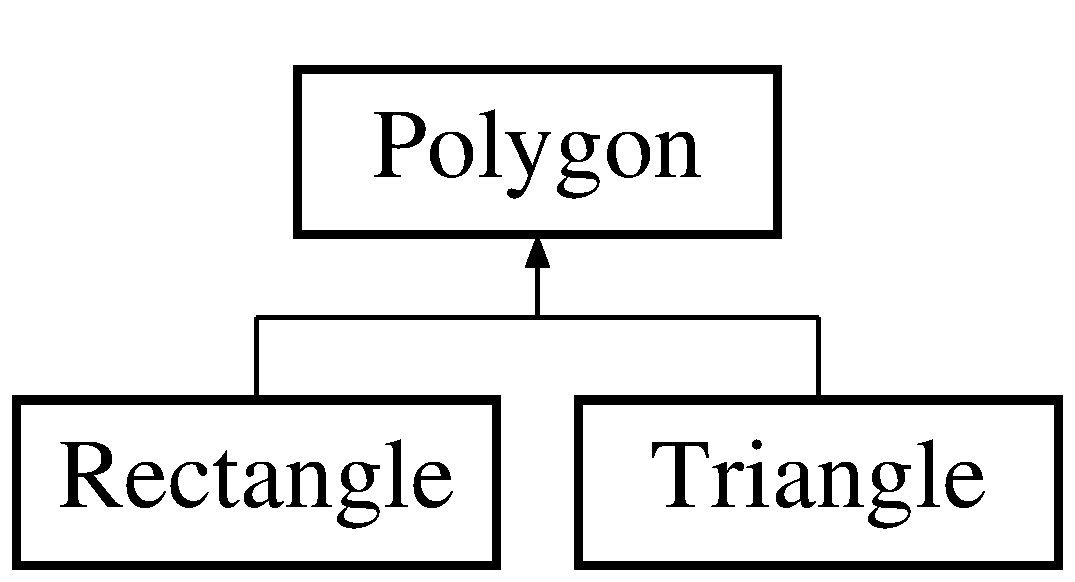
\includegraphics[height=2.000000cm]{class_polygon}
\end{center}
\end{figure}
\subsection*{Public Member Functions}
\begin{DoxyCompactItemize}
\item 
\hyperlink{class_polygon_afb51d4234c64281603f8b11ad23d964e}{Polygon} (const \hyperlink{class_point2_d_array}{Point2\+D\+Array} \&pa, const unsigned int my\+Border\+Color=0xffff, const unsigned int my\+Fill\+Color=0x0000)
\begin{DoxyCompactList}\small\item\em Constructor for the \hyperlink{class_polygon}{Polygon} class. \end{DoxyCompactList}\item 
\hyperlink{class_polygon_a86dc9c4f03f9874f3b1a017b913d50bb}{Polygon} (const \hyperlink{class_point2_d}{Point2\+D} \hyperlink{class_polygon_a3f17a85c09bd04138f22ae31d18b6b4d}{points}\mbox{[}$\,$\mbox{]}, const int num\+Points, const unsigned int my\+Border\+Color=0xffff, const unsigned int my\+Fill\+Color=0x0000)
\begin{DoxyCompactList}\small\item\em Parameter constructor for the the \hyperlink{class_polygon}{Polygon} class. \end{DoxyCompactList}\item 
\hypertarget{class_polygon_ace39c67107966db12e13a183f496c3b0}{\hyperlink{class_polygon_ace39c67107966db12e13a183f496c3b0}{$\sim$\+Polygon} ()}\label{class_polygon_ace39c67107966db12e13a183f496c3b0}

\begin{DoxyCompactList}\small\item\em Destructor for the \hyperlink{class_polygon}{Polygon} class. Decrements num\+Polygons and erases the drawn \hyperlink{class_polygon}{Polygon}. \end{DoxyCompactList}\item 
\hypertarget{class_polygon_a050f5dfd57856852a82a9c7912692d02}{int \hyperlink{class_polygon_a050f5dfd57856852a82a9c7912692d02}{get\+Num\+Sides} ()}\label{class_polygon_a050f5dfd57856852a82a9c7912692d02}

\begin{DoxyCompactList}\small\item\em Gets the number of sides of the \hyperlink{class_polygon}{Polygon} instance. \end{DoxyCompactList}\item 
\hypertarget{class_polygon_a807c06d03f4943e9c8e63a5848ebc5c2}{const \hyperlink{class_point2_d_array}{Point2\+D\+Array} $\ast$ \hyperlink{class_polygon_a807c06d03f4943e9c8e63a5848ebc5c2}{get\+Points} () const }\label{class_polygon_a807c06d03f4943e9c8e63a5848ebc5c2}

\begin{DoxyCompactList}\small\item\em Returns an unmodifiable pointer to the Point\+Array of the \hyperlink{class_polygon}{Polygon}. \end{DoxyCompactList}\item 
void \hyperlink{class_polygon_a91e2048df838eefbf1b291cff13fa540}{set\+Border\+Color} (unsigned int my\+Border\+Color=0xffff)
\begin{DoxyCompactList}\small\item\em Sets the border color of the geometry. \end{DoxyCompactList}\item 
void \hyperlink{class_polygon_ad7caa8108c50e0caf41f286660bbf011}{set\+Fill\+Color} (unsigned int=0x0000)
\begin{DoxyCompactList}\small\item\em Sets the fill color of the geometry. N\+O\+T\+E\+: This needs upgraded in future. \end{DoxyCompactList}\item 
const unsigned int \hyperlink{class_polygon_a89f6cf0b0bc01911b959ada782f9dfd8}{get\+Border\+Color} ()
\begin{DoxyCompactList}\small\item\em Gets the border color of the geometry. \end{DoxyCompactList}\item 
const unsigned int \hyperlink{class_polygon_a1213dc7e01a5c9fc66f0b7190c8b02b6}{get\+Fill\+Color} ()
\begin{DoxyCompactList}\small\item\em Gets the fill color of the geometry. \end{DoxyCompactList}\item 
\hypertarget{class_polygon_a17428a7d7dff4653c905b91020a9f803}{void \hyperlink{class_polygon_a17428a7d7dff4653c905b91020a9f803}{draw} ()}\label{class_polygon_a17428a7d7dff4653c905b91020a9f803}

\begin{DoxyCompactList}\small\item\em Draws the \hyperlink{class_polygon}{Polygon} using the T\+F\+T library. \end{DoxyCompactList}\item 
\hypertarget{class_polygon_aaa6f282cafd882068fae7018741aabaf}{void \hyperlink{class_polygon_aaa6f282cafd882068fae7018741aabaf}{fill} ()}\label{class_polygon_aaa6f282cafd882068fae7018741aabaf}

\begin{DoxyCompactList}\small\item\em Fills the \hyperlink{class_polygon}{Polygon} using the T\+F\+T library. \end{DoxyCompactList}\item 
\hypertarget{class_polygon_a1b7e1ed1a790c4e002b174373fd4a295}{void \hyperlink{class_polygon_a1b7e1ed1a790c4e002b174373fd4a295}{erase} ()}\label{class_polygon_a1b7e1ed1a790c4e002b174373fd4a295}

\begin{DoxyCompactList}\small\item\em Erases the \hyperlink{class_polygon}{Polygon}. \end{DoxyCompactList}\end{DoxyCompactItemize}
\subsection*{Static Public Member Functions}
\begin{DoxyCompactItemize}
\item 
\hypertarget{class_polygon_a1767ac5482d2bd85e8826aacf7214ee5}{static int \hyperlink{class_polygon_a1767ac5482d2bd85e8826aacf7214ee5}{get\+Num\+Polygons} ()}\label{class_polygon_a1767ac5482d2bd85e8826aacf7214ee5}

\begin{DoxyCompactList}\small\item\em Getter method for the number of polygons that have been created. \end{DoxyCompactList}\end{DoxyCompactItemize}
\subsection*{Protected Attributes}
\begin{DoxyCompactItemize}
\item 
\hypertarget{class_polygon_a3f17a85c09bd04138f22ae31d18b6b4d}{\hyperlink{class_point2_d_array}{Point2\+D\+Array} \hyperlink{class_polygon_a3f17a85c09bd04138f22ae31d18b6b4d}{points}}\label{class_polygon_a3f17a85c09bd04138f22ae31d18b6b4d}

\begin{DoxyCompactList}\small\item\em Keeps track of the number of \hyperlink{class_polygon}{Polygon} objects. \end{DoxyCompactList}\item 
\hypertarget{class_polygon_ac7e55927e6dda8a8ef0a9bf937564015}{unsigned int \hyperlink{class_polygon_ac7e55927e6dda8a8ef0a9bf937564015}{border\+Color}}\label{class_polygon_ac7e55927e6dda8a8ef0a9bf937564015}

\begin{DoxyCompactList}\small\item\em Vertices for the \hyperlink{class_polygon}{Polygon} instance. \end{DoxyCompactList}\item 
\hypertarget{class_polygon_a8785a91a1462e4fd02cff574e51f3948}{unsigned int \hyperlink{class_polygon_a8785a91a1462e4fd02cff574e51f3948}{fill\+Color}}\label{class_polygon_a8785a91a1462e4fd02cff574e51f3948}

\begin{DoxyCompactList}\small\item\em Border color of the \hyperlink{class_polygon}{Polygon}. \end{DoxyCompactList}\end{DoxyCompactItemize}
\subsection*{Static Protected Attributes}
\begin{DoxyCompactItemize}
\item 
\hypertarget{class_polygon_a2dc44114b25b8ee2351b3253ccf66376}{static int {\bfseries num\+Polygons} = 0}\label{class_polygon_a2dc44114b25b8ee2351b3253ccf66376}

\end{DoxyCompactItemize}


\subsection{Detailed Description}
Base class for drawing \hyperlink{class_polygon}{Polygon} objects to the T\+F\+T touch screen. 

\subsection{Constructor \& Destructor Documentation}
\hypertarget{class_polygon_afb51d4234c64281603f8b11ad23d964e}{\index{Polygon@{Polygon}!Polygon@{Polygon}}
\index{Polygon@{Polygon}!Polygon@{Polygon}}
\subsubsection[{Polygon}]{\setlength{\rightskip}{0pt plus 5cm}Polygon\+::\+Polygon (
\begin{DoxyParamCaption}
\item[{const {\bf Point2\+D\+Array} \&}]{pa, }
\item[{const unsigned int}]{my\+Border\+Color = {\ttfamily 0xffff}, }
\item[{const unsigned int}]{my\+Fill\+Color = {\ttfamily 0x0000}}
\end{DoxyParamCaption}
)}}\label{class_polygon_afb51d4234c64281603f8b11ad23d964e}


Constructor for the \hyperlink{class_polygon}{Polygon} class. 


\begin{DoxyParams}{Parameters}
{\em \&pa} & The \hyperlink{class_point2_d_array}{Point2\+D\+Array} that defines the vertices of the \hyperlink{class_polygon}{Polygon}. \\
\hline
{\em my\+Border\+Color} & The border color of the rectangle. Default is W\+H\+I\+T\+E. \\
\hline
{\em my\+Fill\+Color} & The fill color of the rectangle. Default is B\+L\+A\+C\+K. \\
\hline
\end{DoxyParams}
\hypertarget{class_polygon_a86dc9c4f03f9874f3b1a017b913d50bb}{\index{Polygon@{Polygon}!Polygon@{Polygon}}
\index{Polygon@{Polygon}!Polygon@{Polygon}}
\subsubsection[{Polygon}]{\setlength{\rightskip}{0pt plus 5cm}Polygon\+::\+Polygon (
\begin{DoxyParamCaption}
\item[{const {\bf Point2\+D}}]{points\mbox{[}$\,$\mbox{]}, }
\item[{const int}]{num\+Points, }
\item[{const unsigned int}]{my\+Border\+Color = {\ttfamily 0xffff}, }
\item[{const unsigned int}]{my\+Fill\+Color = {\ttfamily 0x0000}}
\end{DoxyParamCaption}
)}}\label{class_polygon_a86dc9c4f03f9874f3b1a017b913d50bb}


Parameter constructor for the the \hyperlink{class_polygon}{Polygon} class. 


\begin{DoxyParams}{Parameters}
{\em points\mbox{[}$\,$\mbox{]}} & Array of \hyperlink{class_point2_d}{Point2\+D} objects that define the vertices of the \hyperlink{class_polygon}{Polygon}. \\
\hline
{\em num\+Points} & The number of vertices of the \hyperlink{class_polygon}{Polygon}. \\
\hline
{\em my\+Border\+Color} & The border color of the rectangle. Default is W\+H\+I\+T\+E. \\
\hline
{\em my\+Fill\+Color} & The fill color of the rectangle. Default is B\+L\+A\+C\+K. \\
\hline
\end{DoxyParams}


\subsection{Member Function Documentation}
\hypertarget{class_polygon_a89f6cf0b0bc01911b959ada782f9dfd8}{\index{Polygon@{Polygon}!get\+Border\+Color@{get\+Border\+Color}}
\index{get\+Border\+Color@{get\+Border\+Color}!Polygon@{Polygon}}
\subsubsection[{get\+Border\+Color}]{\setlength{\rightskip}{0pt plus 5cm}const unsigned int Polygon\+::get\+Border\+Color (
\begin{DoxyParamCaption}
{}
\end{DoxyParamCaption}
)}}\label{class_polygon_a89f6cf0b0bc01911b959ada782f9dfd8}


Gets the border color of the geometry. 

\begin{DoxyReturn}{Returns}
Border color of the geometry. 
\end{DoxyReturn}
\hypertarget{class_polygon_a1213dc7e01a5c9fc66f0b7190c8b02b6}{\index{Polygon@{Polygon}!get\+Fill\+Color@{get\+Fill\+Color}}
\index{get\+Fill\+Color@{get\+Fill\+Color}!Polygon@{Polygon}}
\subsubsection[{get\+Fill\+Color}]{\setlength{\rightskip}{0pt plus 5cm}const unsigned int Polygon\+::get\+Fill\+Color (
\begin{DoxyParamCaption}
{}
\end{DoxyParamCaption}
)}}\label{class_polygon_a1213dc7e01a5c9fc66f0b7190c8b02b6}


Gets the fill color of the geometry. 

\begin{DoxyReturn}{Returns}
Fill color of the geometry. 
\end{DoxyReturn}
\hypertarget{class_polygon_a91e2048df838eefbf1b291cff13fa540}{\index{Polygon@{Polygon}!set\+Border\+Color@{set\+Border\+Color}}
\index{set\+Border\+Color@{set\+Border\+Color}!Polygon@{Polygon}}
\subsubsection[{set\+Border\+Color}]{\setlength{\rightskip}{0pt plus 5cm}void Polygon\+::set\+Border\+Color (
\begin{DoxyParamCaption}
\item[{unsigned int}]{my\+Border\+Color = {\ttfamily 0xffff}}
\end{DoxyParamCaption}
)}}\label{class_polygon_a91e2048df838eefbf1b291cff13fa540}


Sets the border color of the geometry. 


\begin{DoxyParams}{Parameters}
{\em my\+Border\+Color} & The border color of the geometry. \\
\hline
\end{DoxyParams}
\hypertarget{class_polygon_ad7caa8108c50e0caf41f286660bbf011}{\index{Polygon@{Polygon}!set\+Fill\+Color@{set\+Fill\+Color}}
\index{set\+Fill\+Color@{set\+Fill\+Color}!Polygon@{Polygon}}
\subsubsection[{set\+Fill\+Color}]{\setlength{\rightskip}{0pt plus 5cm}void Polygon\+::set\+Fill\+Color (
\begin{DoxyParamCaption}
\item[{unsigned int}]{my\+Fill\+Color = {\ttfamily 0x0000}}
\end{DoxyParamCaption}
)}}\label{class_polygon_ad7caa8108c50e0caf41f286660bbf011}


Sets the fill color of the geometry. N\+O\+T\+E\+: This needs upgraded in future. 


\begin{DoxyParams}{Parameters}
{\em my\+Fill\+Color} & The fill color of the geometry. \\
\hline
\end{DoxyParams}


The documentation for this class was generated from the following files\+:\begin{DoxyCompactItemize}
\item 
\hyperlink{_touch_screen_geometry_8h}{Touch\+Screen\+Geometry.\+h}\item 
Touch\+Screen\+Geometry.\+cpp\end{DoxyCompactItemize}

\hypertarget{class_rectangle}{\section{Rectangle Class Reference}
\label{class_rectangle}\index{Rectangle@{Rectangle}}
}


Class for handling the geometry rendering and functions for the T\+F\+T Touch Screen.  




{\ttfamily \#include $<$Touch\+Screen\+Geometry.\+h$>$}

Inheritance diagram for Rectangle\+:\begin{figure}[H]
\begin{center}
\leavevmode
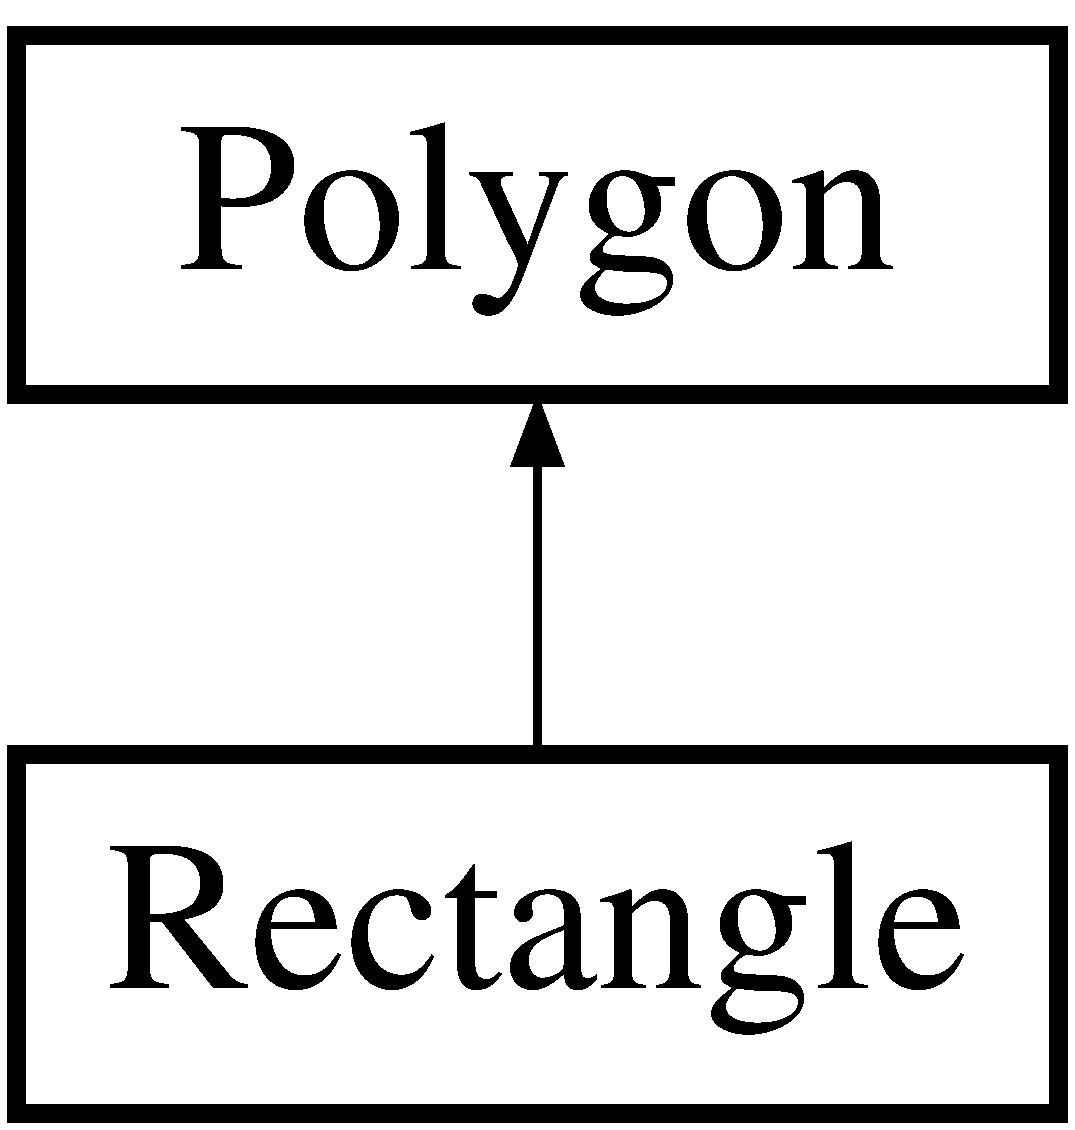
\includegraphics[height=2.000000cm]{class_rectangle}
\end{center}
\end{figure}
\subsection*{Public Member Functions}
\begin{DoxyCompactItemize}
\item 
\hypertarget{class_rectangle_a8a933e0ebd9e80ce91e61ffe87fd577e}{\hyperlink{class_rectangle_a8a933e0ebd9e80ce91e61ffe87fd577e}{Rectangle} ()}\label{class_rectangle_a8a933e0ebd9e80ce91e61ffe87fd577e}

\begin{DoxyCompactList}\small\item\em Default constructor for the \hyperlink{class_rectangle}{Rectangle} class. \end{DoxyCompactList}\item 
\hyperlink{class_rectangle_aed472b7e14717bc8c58bcb18d557fb33}{Rectangle} (\hyperlink{class_point2_d}{Point2\+D} \&upper\+Left, \hyperlink{class_point2_d}{Point2\+D} \&lower\+Right, const unsigned int my\+Border\+Color=0xffff, const unsigned int my\+Fill\+Color=0x0000)
\begin{DoxyCompactList}\small\item\em Parameter constructor for the rectangle subclass. \end{DoxyCompactList}\item 
\hyperlink{class_rectangle_ade5eb36c0149b4e339ccc7e22ab8d25f}{Rectangle} (const int my\+X\+Start, const int my\+Y\+Start, const int my\+Width, const int my\+Height, const unsigned int my\+Border\+Color=0xffff, const unsigned int my\+Fill\+Color=0x0000)
\begin{DoxyCompactList}\small\item\em Parameter constructor for the rectangle subclass. \end{DoxyCompactList}\item 
void \hyperlink{class_rectangle_a35757bfba4460009975a276bab306f28}{set\+Upper\+Left} (const int my\+X\+Start, const int my\+Y\+Start)
\begin{DoxyCompactList}\small\item\em Sets the upper left coordinate of the rectangle while retaining its original height and width. \end{DoxyCompactList}\item 
void \hyperlink{class_rectangle_aa716ed3fddaebd1f13ad1e709642a494}{set\+Values} (const int my\+X\+Start, const int my\+Y\+Start, const int my\+Width, const int my\+Height)
\begin{DoxyCompactList}\small\item\em Sets the values of the rectangle instance. \end{DoxyCompactList}\item 
\hypertarget{class_rectangle_ae2e625affd41dcbb67fa9371cdb73169}{const int \hyperlink{class_rectangle_ae2e625affd41dcbb67fa9371cdb73169}{get\+X\+Start} ()}\label{class_rectangle_ae2e625affd41dcbb67fa9371cdb73169}

\begin{DoxyCompactList}\small\item\em Returns the left bound x-\/coordinate of the rectangle. \end{DoxyCompactList}\item 
\hypertarget{class_rectangle_a3d16a808b34565ad26776b60577e1bf0}{const int \hyperlink{class_rectangle_a3d16a808b34565ad26776b60577e1bf0}{get\+Y\+Start} ()}\label{class_rectangle_a3d16a808b34565ad26776b60577e1bf0}

\begin{DoxyCompactList}\small\item\em Returns the upper bound y-\/coordinate of the rectangle. \end{DoxyCompactList}\item 
\hypertarget{class_rectangle_a748cc274ed586f2a4267cccee4c8aa03}{const int \hyperlink{class_rectangle_a748cc274ed586f2a4267cccee4c8aa03}{get\+X\+End} ()}\label{class_rectangle_a748cc274ed586f2a4267cccee4c8aa03}

\begin{DoxyCompactList}\small\item\em Returns the right bound x-\/coordinate of the rectangle. \end{DoxyCompactList}\item 
\hypertarget{class_rectangle_a05b2d3f5dbf1c0aa92cff4ce6e302f94}{const int \hyperlink{class_rectangle_a05b2d3f5dbf1c0aa92cff4ce6e302f94}{get\+Y\+End} ()}\label{class_rectangle_a05b2d3f5dbf1c0aa92cff4ce6e302f94}

\begin{DoxyCompactList}\small\item\em Returns the lower bound x-\/coordinate of the rectangle. \end{DoxyCompactList}\item 
\hypertarget{class_rectangle_afaea2e6cab12d85e7076e47f092be772}{const int \hyperlink{class_rectangle_afaea2e6cab12d85e7076e47f092be772}{get\+Width} ()}\label{class_rectangle_afaea2e6cab12d85e7076e47f092be772}

\begin{DoxyCompactList}\small\item\em Returns the width of the rectangle. \end{DoxyCompactList}\item 
\hypertarget{class_rectangle_a0fdee2c935c22e3b668e8d1c8e62c8e4}{const int \hyperlink{class_rectangle_a0fdee2c935c22e3b668e8d1c8e62c8e4}{get\+Height} ()}\label{class_rectangle_a0fdee2c935c22e3b668e8d1c8e62c8e4}

\begin{DoxyCompactList}\small\item\em Returns the height of the rectangle. \end{DoxyCompactList}\item 
\hypertarget{class_rectangle_a59d805919cfe95604336afb6e9d54f6f}{void \hyperlink{class_rectangle_a59d805919cfe95604336afb6e9d54f6f}{fill} ()}\label{class_rectangle_a59d805919cfe95604336afb6e9d54f6f}

\begin{DoxyCompactList}\small\item\em Fills the \hyperlink{class_rectangle}{Rectangle} using the T\+F\+T library. \end{DoxyCompactList}\item 
void \hyperlink{class_rectangle_aa6f0b3ca31c9bc2fe7094e1859e22650}{set\+Size} (const int my\+Width, const int my\+Height)
\begin{DoxyCompactList}\small\item\em Sets the size of the rectangle. Does no redraw the rectangle. \end{DoxyCompactList}\item 
void \hyperlink{class_rectangle_a834f54f7040623d8bae999580b02b2b1}{move} (const int dx, const int dy)
\begin{DoxyCompactList}\small\item\em Moves the rectangle at the specified amount. Assumes the specified amount is not outside the screen boundaries. \end{DoxyCompactList}\item 
void \hyperlink{class_rectangle_a823b01fda97c5d8d6252e526c3e1e27e}{scale} (const float factor)
\begin{DoxyCompactList}\small\item\em Resizes the rectangle based on the factor. Assumes the scaling factor is neither too small or too big. \end{DoxyCompactList}\end{DoxyCompactItemize}
\subsection*{Additional Inherited Members}


\subsection{Detailed Description}
Class for handling the geometry rendering and functions for the T\+F\+T Touch Screen. 

\subsection{Constructor \& Destructor Documentation}
\hypertarget{class_rectangle_aed472b7e14717bc8c58bcb18d557fb33}{\index{Rectangle@{Rectangle}!Rectangle@{Rectangle}}
\index{Rectangle@{Rectangle}!Rectangle@{Rectangle}}
\subsubsection[{Rectangle}]{\setlength{\rightskip}{0pt plus 5cm}Rectangle\+::\+Rectangle (
\begin{DoxyParamCaption}
\item[{{\bf Point2\+D} \&}]{upper\+Left, }
\item[{{\bf Point2\+D} \&}]{lower\+Right, }
\item[{const unsigned int}]{my\+Border\+Color = {\ttfamily 0xffff}, }
\item[{const unsigned int}]{my\+Fill\+Color = {\ttfamily 0x0000}}
\end{DoxyParamCaption}
)}}\label{class_rectangle_aed472b7e14717bc8c58bcb18d557fb33}


Parameter constructor for the rectangle subclass. 


\begin{DoxyParams}{Parameters}
{\em upper\+Left} & The upper left vertice of the rectangle. \\
\hline
{\em lower\+Right} & The lower right vertice of the rectangle. \\
\hline
{\em my\+Border\+Color} & The border color of the rectangle. \\
\hline
{\em my\+Fill\+Color} & The fill color of the rectangle. \\
\hline
\end{DoxyParams}
\hypertarget{class_rectangle_ade5eb36c0149b4e339ccc7e22ab8d25f}{\index{Rectangle@{Rectangle}!Rectangle@{Rectangle}}
\index{Rectangle@{Rectangle}!Rectangle@{Rectangle}}
\subsubsection[{Rectangle}]{\setlength{\rightskip}{0pt plus 5cm}Rectangle\+::\+Rectangle (
\begin{DoxyParamCaption}
\item[{const int}]{my\+X\+Start, }
\item[{const int}]{my\+Y\+Start, }
\item[{const int}]{my\+Width, }
\item[{const int}]{my\+Height, }
\item[{const unsigned int}]{my\+Border\+Color = {\ttfamily 0xffff}, }
\item[{const unsigned int}]{my\+Fill\+Color = {\ttfamily 0x0000}}
\end{DoxyParamCaption}
)}}\label{class_rectangle_ade5eb36c0149b4e339ccc7e22ab8d25f}


Parameter constructor for the rectangle subclass. 


\begin{DoxyParams}{Parameters}
{\em my\+X\+Start} & The starting x-\/coordinate of the rectangle. \\
\hline
{\em my\+Y\+Start} & The starting y-\/coordinate of the rectangle. \\
\hline
{\em my\+Width} & The width of the rectangle. \\
\hline
{\em my\+Height} & The height of the rectangle. \\
\hline
{\em my\+Border\+Color} & The border color of the rectangle. \\
\hline
{\em my\+Fill\+Color} & The fill color of the rectangle. \\
\hline
\end{DoxyParams}


\subsection{Member Function Documentation}
\hypertarget{class_rectangle_a834f54f7040623d8bae999580b02b2b1}{\index{Rectangle@{Rectangle}!move@{move}}
\index{move@{move}!Rectangle@{Rectangle}}
\subsubsection[{move}]{\setlength{\rightskip}{0pt plus 5cm}void Rectangle\+::move (
\begin{DoxyParamCaption}
\item[{const int}]{dx, }
\item[{const int}]{dy}
\end{DoxyParamCaption}
)}}\label{class_rectangle_a834f54f7040623d8bae999580b02b2b1}


Moves the rectangle at the specified amount. Assumes the specified amount is not outside the screen boundaries. 


\begin{DoxyParams}{Parameters}
{\em dx} & The amount in the +x-\/direction (left to right) to move the rectangle. \\
\hline
{\em dy} & The amount in the +y-\/direction (up to down) to move the rectangle. \\
\hline
\end{DoxyParams}
\hypertarget{class_rectangle_a823b01fda97c5d8d6252e526c3e1e27e}{\index{Rectangle@{Rectangle}!scale@{scale}}
\index{scale@{scale}!Rectangle@{Rectangle}}
\subsubsection[{scale}]{\setlength{\rightskip}{0pt plus 5cm}void Rectangle\+::scale (
\begin{DoxyParamCaption}
\item[{const float}]{factor}
\end{DoxyParamCaption}
)}}\label{class_rectangle_a823b01fda97c5d8d6252e526c3e1e27e}


Resizes the rectangle based on the factor. Assumes the scaling factor is neither too small or too big. 


\begin{DoxyParams}{Parameters}
{\em factor} & The amount the rectangle is to be resized. \\
\hline
\end{DoxyParams}
\hypertarget{class_rectangle_aa6f0b3ca31c9bc2fe7094e1859e22650}{\index{Rectangle@{Rectangle}!set\+Size@{set\+Size}}
\index{set\+Size@{set\+Size}!Rectangle@{Rectangle}}
\subsubsection[{set\+Size}]{\setlength{\rightskip}{0pt plus 5cm}void Rectangle\+::set\+Size (
\begin{DoxyParamCaption}
\item[{const int}]{my\+Width, }
\item[{const int}]{my\+Height}
\end{DoxyParamCaption}
)}}\label{class_rectangle_aa6f0b3ca31c9bc2fe7094e1859e22650}


Sets the size of the rectangle. Does no redraw the rectangle. 


\begin{DoxyParams}{Parameters}
{\em my\+Width} & The width of the rectangle. \\
\hline
{\em my\+Height} & The height of the rectangle. \\
\hline
\end{DoxyParams}
\hypertarget{class_rectangle_a35757bfba4460009975a276bab306f28}{\index{Rectangle@{Rectangle}!set\+Upper\+Left@{set\+Upper\+Left}}
\index{set\+Upper\+Left@{set\+Upper\+Left}!Rectangle@{Rectangle}}
\subsubsection[{set\+Upper\+Left}]{\setlength{\rightskip}{0pt plus 5cm}void Rectangle\+::set\+Upper\+Left (
\begin{DoxyParamCaption}
\item[{const int}]{my\+X\+Start, }
\item[{const int}]{my\+Y\+Start}
\end{DoxyParamCaption}
)}}\label{class_rectangle_a35757bfba4460009975a276bab306f28}


Sets the upper left coordinate of the rectangle while retaining its original height and width. 


\begin{DoxyParams}{Parameters}
{\em my\+X\+Start} & The left bound x-\/coordinate of the rectangle. \\
\hline
{\em my\+Y\+Start} & The upper bound y-\/coodinate of the rectangle. \\
\hline
\end{DoxyParams}
\hypertarget{class_rectangle_aa716ed3fddaebd1f13ad1e709642a494}{\index{Rectangle@{Rectangle}!set\+Values@{set\+Values}}
\index{set\+Values@{set\+Values}!Rectangle@{Rectangle}}
\subsubsection[{set\+Values}]{\setlength{\rightskip}{0pt plus 5cm}void Rectangle\+::set\+Values (
\begin{DoxyParamCaption}
\item[{const int}]{my\+X\+Start, }
\item[{const int}]{my\+Y\+Start, }
\item[{const int}]{my\+Width, }
\item[{const int}]{my\+Height}
\end{DoxyParamCaption}
)}}\label{class_rectangle_aa716ed3fddaebd1f13ad1e709642a494}


Sets the values of the rectangle instance. 


\begin{DoxyParams}{Parameters}
{\em my\+X\+Start} & The starting x-\/coordinate of the rectangle. \\
\hline
{\em my\+Y\+Start} & The starting y-\/coordinate of the rectangle. \\
\hline
{\em my\+Width} & The width of the rectangle. \\
\hline
{\em my\+Height} & The height of the rectangle. \\
\hline
\end{DoxyParams}


The documentation for this class was generated from the following files\+:\begin{DoxyCompactItemize}
\item 
\hyperlink{_touch_screen_geometry_8h}{Touch\+Screen\+Geometry.\+h}\item 
Touch\+Screen\+Geometry.\+cpp\end{DoxyCompactItemize}

\hypertarget{class_triangle}{\section{Triangle Class Reference}
\label{class_triangle}\index{Triangle@{Triangle}}
}


Class for drawing Triangles to the T\+F\+T touch screen.  




{\ttfamily \#include $<$Touch\+Screen\+Geometry.\+h$>$}

Inheritance diagram for Triangle\+:\begin{figure}[H]
\begin{center}
\leavevmode
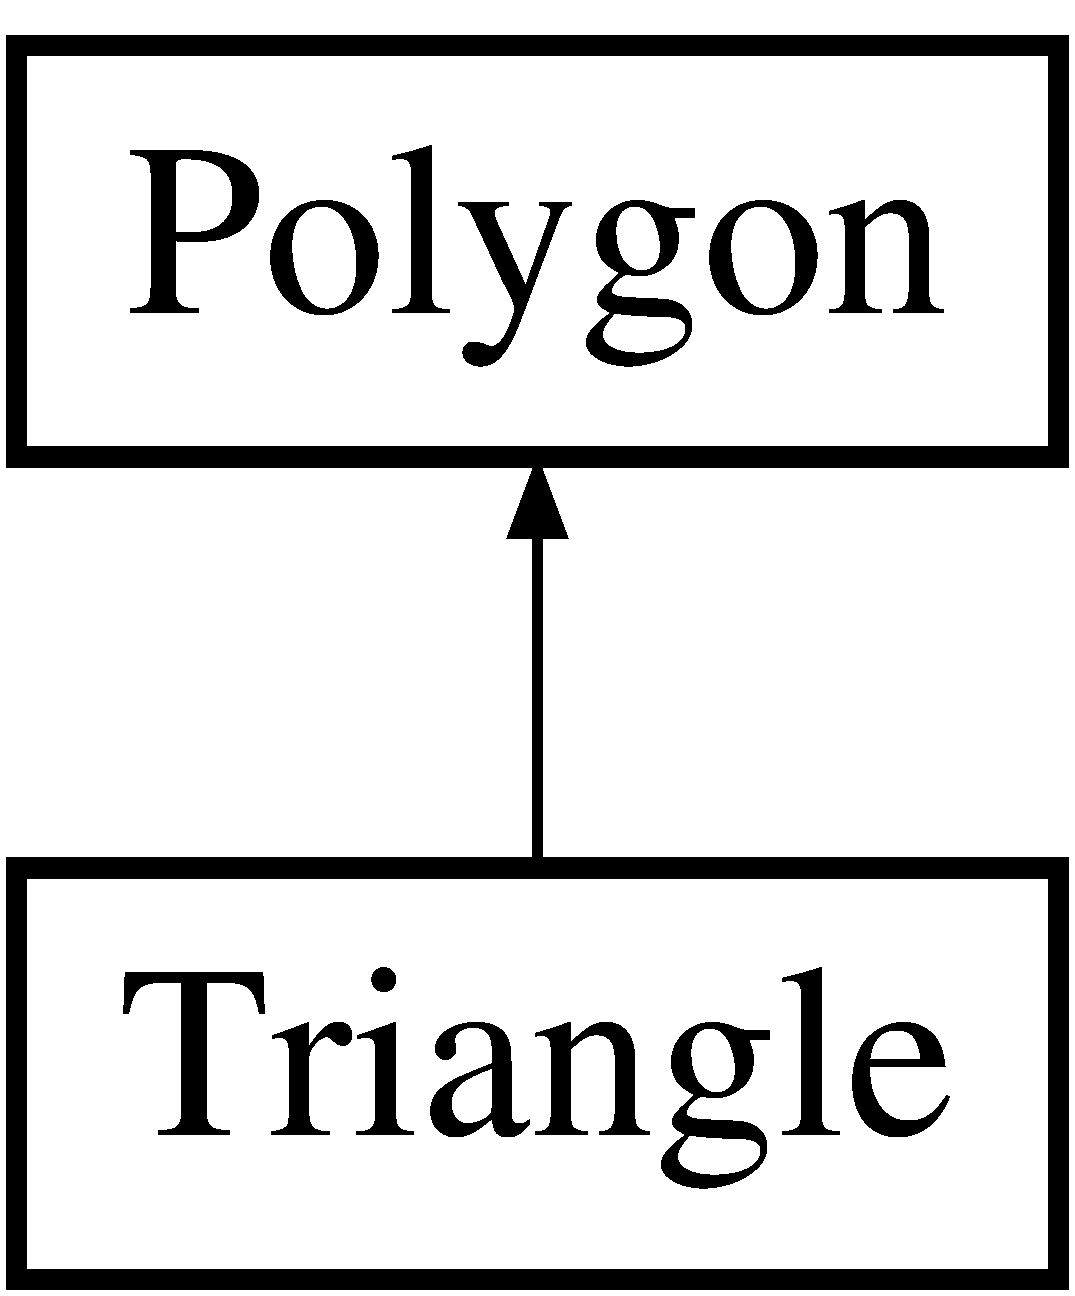
\includegraphics[height=2.000000cm]{class_triangle}
\end{center}
\end{figure}
\subsection*{Public Member Functions}
\begin{DoxyCompactItemize}
\item 
\hyperlink{class_triangle_a477c11aa9dfce48a502e535874474fec}{Triangle} (const \hyperlink{class_point2_d}{Point2\+D} \&a, const \hyperlink{class_point2_d}{Point2\+D} \&b, const \hyperlink{class_point2_d}{Point2\+D} \&c, const unsigned int my\+Border\+Color=0xffff, const unsigned int my\+Fill\+Color=0x0000)
\begin{DoxyCompactList}\small\item\em Parameter constructor for the \hyperlink{class_triangle}{Triangle} class. \end{DoxyCompactList}\end{DoxyCompactItemize}
\subsection*{Additional Inherited Members}


\subsection{Detailed Description}
Class for drawing Triangles to the T\+F\+T touch screen. 

\subsection{Constructor \& Destructor Documentation}
\hypertarget{class_triangle_a477c11aa9dfce48a502e535874474fec}{\index{Triangle@{Triangle}!Triangle@{Triangle}}
\index{Triangle@{Triangle}!Triangle@{Triangle}}
\subsubsection[{Triangle}]{\setlength{\rightskip}{0pt plus 5cm}Triangle\+::\+Triangle (
\begin{DoxyParamCaption}
\item[{const {\bf Point2\+D} \&}]{a, }
\item[{const {\bf Point2\+D} \&}]{b, }
\item[{const {\bf Point2\+D} \&}]{c, }
\item[{const unsigned int}]{my\+Border\+Color = {\ttfamily 0xffff}, }
\item[{const unsigned int}]{my\+Fill\+Color = {\ttfamily 0x0000}}
\end{DoxyParamCaption}
)}}\label{class_triangle_a477c11aa9dfce48a502e535874474fec}


Parameter constructor for the \hyperlink{class_triangle}{Triangle} class. 


\begin{DoxyParams}{Parameters}
{\em a} & The 1st vertice of the triangle. \\
\hline
{\em b} & The 2nd vertice of the triangle. \\
\hline
{\em c} & The 3rd vertice of the triangle. \\
\hline
{\em my\+Border\+Color} & The border color of the triangle. Default is white. \\
\hline
{\em my\+Fill\+Color} & The fill color of the rectangle. Default is black. \\
\hline
\end{DoxyParams}


The documentation for this class was generated from the following files\+:\begin{DoxyCompactItemize}
\item 
\hyperlink{_touch_screen_geometry_8h}{Touch\+Screen\+Geometry.\+h}\item 
Touch\+Screen\+Geometry.\+cpp\end{DoxyCompactItemize}

\chapter{File Documentation}
\hypertarget{_touch_screen_geometry_8h}{\section{Touch\+Screen\+Geometry.\+h File Reference}
\label{_touch_screen_geometry_8h}\index{Touch\+Screen\+Geometry.\+h@{Touch\+Screen\+Geometry.\+h}}
}


Library for creating geometries shapes for the Seeed Studio T\+F\+T touch screen.  


{\ttfamily \#include \char`\"{}Arduino.\+h\char`\"{}}\\*
\subsection*{Classes}
\begin{DoxyCompactItemize}
\item 
class \hyperlink{class_point2_d}{Point2\+D}
\begin{DoxyCompactList}\small\item\em Abstract data type for representing a point in the 2\+D cartesian plane. \end{DoxyCompactList}\item 
class \hyperlink{class_point2_d_array}{Point2\+D\+Array}
\begin{DoxyCompactList}\small\item\em Abstract data class for arrays of \hyperlink{class_point2_d}{Point2\+D} objects. \end{DoxyCompactList}\item 
class \hyperlink{class_polygon}{Polygon}
\begin{DoxyCompactList}\small\item\em Base class for drawing \hyperlink{class_polygon}{Polygon} objects to the T\+F\+T touch screen. \end{DoxyCompactList}\item 
class \hyperlink{class_rectangle}{Rectangle}
\begin{DoxyCompactList}\small\item\em Class for handling the geometry rendering and functions for the T\+F\+T Touch Screen. \end{DoxyCompactList}\item 
class \hyperlink{class_triangle}{Triangle}
\begin{DoxyCompactList}\small\item\em Class for drawing Triangles to the T\+F\+T touch screen. \end{DoxyCompactList}\item 
class \hyperlink{class_circle}{Circle}
\begin{DoxyCompactList}\small\item\em The class for drawing circles to the T\+F\+T touch screen. \end{DoxyCompactList}\end{DoxyCompactItemize}


\subsection{Detailed Description}
Library for creating geometries shapes for the Seeed Studio T\+F\+T touch screen. 

\begin{DoxyAuthor}{Author}
Richard Kirkpatrick 
\end{DoxyAuthor}
\begin{DoxyDate}{Date}
17 July 2014
\end{DoxyDate}
Copyright\+: This material is heavility influenced by material from M\+I\+T Open\+Course\+Ware which operates under a Creative Common License. For more info, visit \href{http://ocw.mit.edu/terms/}{\tt http\+://ocw.\+mit.\+edu/terms/}

All other material (Rectangle\+Array, Circle\+Array, draw() and fill() methods ...) was created by myself. Please follow the Open\+Source guidelines and P\+L\+E\+A\+S\+E give credit to M\+I\+T Open\+Course\+Ware and myself when using this work. 
%--- End generated contents ---

% Index
\newpage
\phantomsection
\addcontentsline{toc}{chapter}{Index}
\printindex

\end{document}
